\documentclass[a4paper]{article}
\usepackage[T1]{fontenc}
\usepackage[utf8]{inputenc}
\usepackage{lmodern}
\usepackage{graphicx}
\usepackage{hyperref}
\usepackage{tabulary}
\usepackage{lscape}

\usepackage[
			portrait,
			bindingoffset=1.5cm,
			inner=2.5cm,
			outer=2.5cm,
			top=3cm,
			bottom=3cm
				]{geometry}
\usepackage{float}
\restylefloat{table}
\usepackage{wrapfig}
\usepackage[
backend=biber,
style=numeric,
sorting=ynt
]{biblatex}
\addbibresource{references.bib}
\usepackage{setspace} 
\DeclareUnicodeCharacter{00A0}{ }

\urldef{\AJAX}\url{https://en.wikipedia.org/wiki/Ajax_(programming)}
\urldef{\DROPBOX}\url{https://www.dropbox.com/}

\begin{document}
\begin{titlepage}

\newcommand{\HRule}{\rule{\linewidth}{0.7mm}} % Defines a new command for the horizontal lines, change thickness here


\center % Center everything on the page
 
%----------------------------------------------------------------------------------------
%	HEADING SECTIONS
%----------------------------------------------------------------------------------------

\textsc{\LARGE University of Tromsø}\\[1.5cm] % Name of your university/college
\textsc{\Large INF-2900}\\[0.5cm] % Major heading such as course name
\textsc{\large Software Engineering}\\[3cm] % Minor heading such as course title

%----------------------------------------------------------------------------------------
%	TITLE SECTION
%----------------------------------------------------------------------------------------

\includegraphics[scale=0.25]{pictures/turi_logo.png}\\[0.5cm]
{ \huge \bfseries Turi}\\[2cm] % Title of your document
 
%----------------------------------------------------------------------------------------
%	AUTHOR SECTION
%----------------------------------------------------------------------------------------


% If you don't want a supervisor, uncomment the two lines below and remove the section above
\Large \emph{Group: 1}\\[1.5cm]
% title
%----------------------------------------------------------------------------------------
%	DATE SECTION
%----------------------------------------------------------------------------------------

\textsc{\large Spring 2015}\\[2cm] % Date, change the \today to a set date if you want to be precise

%----------------------------------------------------------------------------------------
%	LOGO SECTION
%----------------------------------------------------------------------------------------

\includegraphics{pictures/UiT_samarbeidslogo_bokmal_300ppi.png}\\[1cm] 
% Include a department/university logo - this will require the graphicx package
 
%----------------------------------------------------------------------------------------

\vfill % Fill the rest of the page with whitespace

\end{titlepage}
% END TITLE PAGE %

\tableofcontents
\pagebreak


\section{Introduction}
Imagine you want to go on a trip - to Norway for example. You ask you friends to join you but they reject because they can not afford the money or they have no spare time. What now?

You can either go alone or try to find some people who can join you. The first place we look today is on the world wide web. We already can find some portals where you can find partners for your trip. But what about planning your actually trip?

We couldn’t find a tool which allows you to plan your trip in detail. Planning your trip gets especially difficult if you find your trip mates online and you can not meet because you live too far away from each other. 

You can now either use the phone or create e.g. some Facebook group. Still those ways lack of several features we want to implement in our trip planner which makes it unique. In fact we came up with the idea to create a a trip planner which offers a combination between socialising and planning for your trips.\\

\begin{figure}[!h]
  \begin{center}
    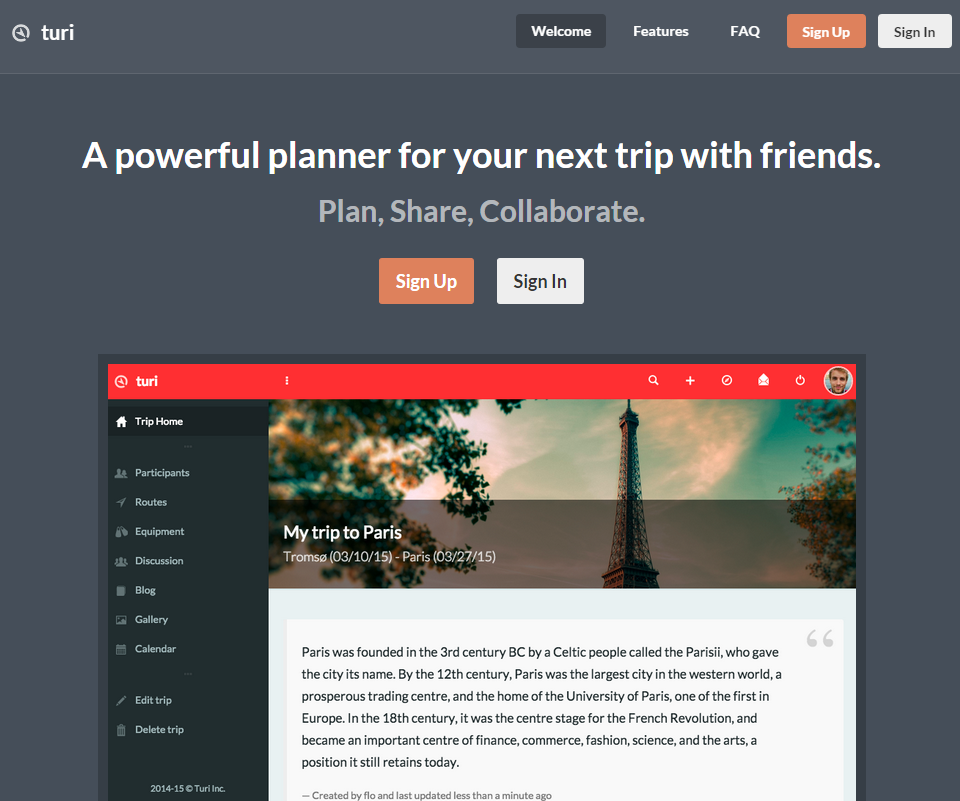
\includegraphics[width=1\textwidth]{pictures/turi_landing_page.png}
  \end{center}
\caption{Turi Landing Page}
\label{fig:turilandingpage}
\end{figure}

\subsection{The product name: turi}
The name derived from the Norwegian word “tur” (a trip/a walk). turi was short and concise enough and sounds good to the ear. It is also a Norwegian name, but this will be no problem when we think about topics like a trademark etc.

\subsection{Setup and Live Demo}

With this report we delivered you the latest turi sources. To run the project just follow the steps in the README.md file in the root folder of the project. However you can checkout the latest sources also from our GitHub repository (\url{https://github.com/turi-inc/turi/}).\\

As a third option we uploaded a fully functional snapshot of the latest changes (we reset the snapshot after every push to our develop branch): \url{https://turi.herokuapp.com}

\subsection{Summary of goals (planned functionalities)}
The following functionalities should be supported (bold means that we they were implemented during the course sprints):
\begin{itemize}
  \item {\textbf{Discuss with participants}}
  \item {\textbf{Event management (for appointments top plan)}}
  \item {\textbf{Route planning}}
  \item {\textbf{Equipment planning}}
  \item {\textbf{Gallery to visualize your trip experiences}}
  \item {\textbf{Blog about your experience}}
  \item {\textbf{Share your trip (public/private)}}
  \item {Copy a previous trip from others (e.g. routes)}
  \item {Rating functionality and other common social functions (commenting, likes..)
  \begin{itemize}
    \item {\textbf{Friend requests}}
  \end{itemize}}
  \item {\textbf{Explore trips based on their location}}
  \item {Badges and rewards for participating and using Turi}
  \item {Search and find trips according your interests}
\end{itemize}

\noindent
In the end we weren't able to implement all of our goals (the goals which are not in bold) and we had tons of more ideas. But for the first release of turi (1.0.0) we decided to require all these features above.\\

\section{Theme and Design}
The theme should be minimalistic and consistent. Therefore we decided to go with a existing theme and implement our features. We've gone with a theme named "AppUI"\footnote{http://themeforest.net/item/appui-web-app-bootstrap-admin-template/8603616}. It's available on the online platform "themeforest". It already includes a lot of sample pages so we only had to replace those placeholder widgets with our own views and partials.

\section{Gems}
We use several gems in our project, this means that we didn't need to reinvent the wheel for features that already exist, and we could focus on our own features. All the gems used can be found in the gemfile in the project source, but the most important ones are the following.
\subsection{Devise}
Devise is a popular authentication solution for Rails based on Warden \cite{devise}. \\
In the first iterations we created our own authentication system, but we found out that we could use \textit{Devise}, after the lecture about authentication. This made it possible to focus more on other task in the project, and less on the details of making a secure and safe authentication system. 

\subsection{Pundit}
\textit{Pundit} is an authorization system\cite{pundit}, which we use in almost all of the features in the project. Our main usage of the gem is to check privileges when a user interacts with the trip or the trip features. For example an editor and the owner of a trip are able to edit the trip title, description and so on, but a viewer is not able to do this. 

\subsection{Leaflet}
\textit{Leaflet}\cite{leaflet} is a JavaScript library that let us implement the interactive map for the routes. Before discovering \textit{Leaflet}, we looked at a similar gem from Google, but it was too heavy for our requirements. As an example, Google Maps seemed to snap waypoints to the nearest road, which is counter-productive for us since we want the users to be able to plan any kind of trip, including hikes.

\subsection{rails-assets}
Rails assets\footnote{https://rails-assets.org/} are used to include common JavaScript libraries which extend mainly jQuery and Bootstrap. Using the rails assets source, we can benefit from pre packaged JavaScript libraries which are automatically included in the rails asset pipeline.

\subsection{Geocoder}
\textit{Geocoder} is a so called "complete geocoding solution for Ruby"\cite{geocoder}, it provides a location based on IP, location and so on, in the project we use it for location based search, for example in the trip start and end location to show the location in the explore map. 

\subsection{Puma}
\textit{Puma} is a "simple, fast, threaded, and highly concurrent HTTP 1.1 server for Ruby/Rack applications."\cite{puma}. Heroku recommend \textit{Puma} over the stock rails server (WEBrick) by saying that: "While WEBrick should be fine for development, it was not designed to handle a high concurrent workload that a Ruby app must serve in production. A production web server should be used instead."\cite{heroku}. Even though Heroku only uses one core (for the free program), this ensures that the project is ready for deployment onto a multi-core server in the future.  


\section{Trip Features}
The trip and it's features are the main focus of our project. 
\subsection{Discussion}

\begin{figure}[!h]
  \begin{center}
    \vspace{-0pt}
    \includegraphics[width=0.5\textwidth]{pictures/discussion}
  \end{center}
\caption{Turi discussion}
\label{fig:discussion}
\end{figure}

This feature is for discussion among the trip participants. If something needs discussion considering the trip, this is a place where the participants can come to an agreement. All participants can create a new discussion and comment on others and their own discussions. Figure \ref{fig:discussion} is an example of the discussion feature. At the top of the figure is the title of discussion. Next to it is the name of the discussion creator and how long since it was created. Below the title are the comments to the discussion. Each comment has information on who created it, how long since it was created and an image of the creator, if available. Adding new comments to the discussion is done by exchanging data to the server using AJAX \footnote{\AJAX}. This gives a smoother experience for the commentator. 

\subsection{Event management}
The event management is a simple calender where you can add events. We make usage of a jQuery Plugin called "fullCalendar" which does all the frontend logic for us. In the backend we simply store events with a date and description etc. The events are then pulled via AJAX by fullCalendar and a small JSON interface in our EventController.

\subsection{Equipment planning}
Equipment planning is essential for a trip, knowing what you need to bring and the ability to distribute responsibilities between the participants of the trip. In our implementation each trip can have multiple list, which can contain multiple items. Each item in return contains a number (number of items) and a price, these items can be assigned to other participants. Charts provide an overview of all the lists and for each individual list, these charts provide a summary of the assignments (items and price) for each participant in a pie chart. \\ This feature had two different user stories attached to it (see Appendix A, table \ref{tab:sprint2}, number 4 and 5), and they had a combined point value of 13. This estimation was reasonable, and the implementation of the features spanned the entire second sprint. We changed the look and feel of the features multiple during this sprint, before ending up at the current implementation, which we felt was the most intuitive. There weren't any particular problems we faced when implementing this feature. There was, however, a lot of work to get everything working on a single view page, instead of having views for each of the controllers. A particularly tricky part of the feature was the form for the item assignment, since we used the same form for creating, editing and deleting, this caused the create method of the equipment-assignment controller to become quite large and complex. 

\subsection{Gallery}
The gallery feature enables the integration of Dropbox \footnote{\DROPBOX}. The user gives us the right to see his images. But of course we wanted to let the customer still feel safe. Therefore he has to create a new Dropbox folder called "turi". When he connects Dropbox to a trip he also has to create a subfolder in "turi" after his trip name. So if you call your trip e.g. "My Trip to London" we will display all images of the user under the folder "turi/my\_trip\_to\_london" to all trip participants. The public feature will allow you in the near future to declare a public folder like "turi/my\_trip\_to\_london/public". This folder will be visible on the public trip page to show external users some impressions of the trip. Beside that the user can always revoke his Dropbox acces by simply clicking the bin icon on the trip gallery page. It should be mentioned that the Dropbox Api is stubbed during the tests since we wanted to make sure that turi can be tested offline.

\subsection{Blog}
The blog platform allows a trip editor to create a blog associated with the trip. The user can edit the blog through a simple editor interface which also allows for URLs and images. A blog can be marked as public, which means that non-participants can read it. The platform has a blog index list which lists the blogs in order of creation and shows an excerpt from each entry.\\

\noindent
The text input is handled through a plug-in named CKEditor\cite{ckeditor}. This plug-in integrates with a text area and allows the user to work with text in a similar fashion as a regular text editor It automatically adds the appropriate HTML tags necessary to render the text properly in a browser. By default the editor has an overwhelming amount of tools available, but for this implementation the number of tools has been greatly reduced to remove unneeded functions and improve ease-of-use.\\

\noindent
In general, implementing the blog was straight-forward to implement and the only issues that presented themselves were designing the tests and getting the interface to look presentable. The blog was assigned a single user story estimated at 5 points, which in retrospect seems fairly appropriate.

\subsection{Share your trip (public setting)}
A trip is private to the participants of the trip, unless they decide it should be shared with the public. The public should only be able to view a small subset of the information about the trip, which the participants agree to share. Therefore each trip needs a private setting and its own public view, this was the one of the main things we wanted to implement in the 3rd sprint for the project. \\

\noindent
The implementation of the feature was quite straightforward. The thing that took the most time was the design of the public trip view, and finding out what and how we were going to show the different elements on a single page. We ended up using \emph{Kaminari}\cite{kaminari}, to "paginate" the different elements. For example if a trip has many public blog entries, only one of them are displayed on the page at any given time. 

\subsection{Explore trips}
The explore trip feature was one of our last implementations. We provide a fullscreen map which fetches all public trips via AJAX and display them on the map.Furthermore we added a plug-in that groups trips based on their locations so you have to zoom in or click on the trip group to see all the trips available for this specific area.

\subsection{Search}
The search system is implemented through address tags which are read out of a form and appended on the address bar. These tags are read as arguments by the controller methods running search, and are used to do look-up in the database. The search allows the user to do a search on title, start and end location and date, and tags. The same engine is also used to search for other users.\\

\noindent
Making a search engine for trips made it necessary to consider what the user would want to search for. A trip has several data fields but not every field makes for a useful search option. A search on location is useful in that it find trips related to a certain location, while a search on description leaves few guarantees for what the result will be. The final implementation allows for search on title, start and end locations and dates, and tags. A possible missing option could be to search for trips created by a specific user, although this is not necessarily needed since the engine also allows for searching for specific users.\\

\noindent
The solution used here is not the only possible solution. A second option would be to use a separate model and controller for search. This allows for storing searches and makes the logic behind the implementation cleaner, depending on the number of fields used as search terms. The downside is extra logic is needed to clean the database of old searches regularly. Since each search is its own entry, it could end up growing much faster than any of the other databases. The solution used is simpler, but faster to implement and the difference in user experience is minimal.\\

\noindent
The search system was assigned a single user story estimated at 8 points. The scoring of the story seemed appropriate as implementing search required some time to study the different options available and implement it. Not every field could be read through the same query which meant extra work for comparison and merging of search results before getting the final result. This led to some trial and error to get the query results correct. Unfortunately the user story in question only refers to searching for trips and not users and no additional user stories were made for the user search. This means that there is no tracking available for the work done on the user search and no estimation for work load.


\subsection{Route Planner}

\begin{figure}[!h]
  \begin{center}
    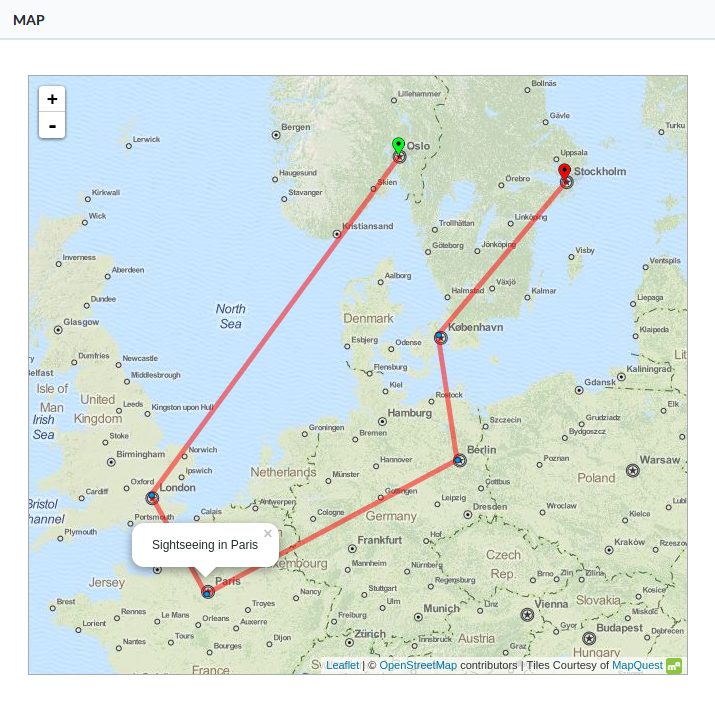
\includegraphics[width=1\textwidth]{pictures/route_planning}
  \end{center}
\caption{Turi Route Planner}
\label{fig:route}
\end{figure}

\noindent
When planning a trip, it could be very useful to illustrate the route, and points of interests on a map. This map should be visible to all the participants so that the route, or proposed route, could be discussed.\\

\noindent
Bjørnar and Kristoffer was given the responsibility of implementing the feature, and when planning the second sprint a single user story (see Appendix A, table \ref{tab:sprint3}, number 5) was created for the entire feature. The user story was given the maximum points for complexity by the scrum poker session, thus it was expected that the entire feature was to be implemented during the second sprint. \\

\noindent
In retrospect, the user story could have been classified as an “epic”, with multiple fine-grained user stories. The implementation could have been divided into three main parts; the map control and GUI, the back-end model and controller, and the view. And given how the workload have been on this feature, we would have given the map control 13 points, the back-end, including tests would get 8 points, and the view would get about 3 points. \\

\noindent
Implementing the feature was mainly done by pair-programming. This worked really well for the map, which was implemented in JavaScript, using the Leaflet API, where one was writing code, and the other was helping, and could very quickly look up manuals and documentation on the fly. \\

\noindent
The model and controller were a bit more complicated for this feature, than for the other features. A route is a collection of waypoints, and at first, we thought about having these as two separate models, but after some help from Runar, we decided on a structure where the route model uses nested-attributes of the waypoint model. This means that waypoints are passed as parameters of a route upon its creation instead of being appended after the fact. \\

\noindent
We did not put much effort into the view during the implementation of the feature, and at the end, we did not feel this was a bad choice, since the group did not decide on a uniform design before the end of the third sprint. And since Florian had put a lot of work into the layouts, applying a design to the views was trivial. \\

\noindent
The feature was implemented on a separate branch on Github, and was only merged into the development branch at the end of the third sprint, when the feature was done. This was not a deliberate choice, but the view was always a work in progress, and we did not feel the feature was polished enough to be introduced in the master branch. There was also the continuous development functionality, that required that all tests needed to pass before a pull request could be accepted, and we did not start writing tests until at the end of the third sprint. \\

\section{Other features}
\subsection{Friend requests}
Now that you have registered and logged into the turi site and been on a trip with some people and now you want to continue to stay in touch with them so that you can go with more trips with them. This is why the friendship feature was created, so that you as a user have the option to add other users as your friends. \\

\noindent
The user story for the friends feature was made in the second sprint and it was given 5 points during the scrum poker session. Ingvild was given the responsibility for implementing the friends feature. In the beginning this feature was implemented without friend requests. In the third sprint the ability to request friendship was added. This time both Runar and Ingvild was assigned to work on the request. But it was not given a an user story since it was a part of the friends user story. In retrospect this user story should have been given 8 points since there was some work with friends and request. \\

\noindent
When a user clicks "add friend", rails will build a request for the user id and the receiver id. The pending request will come up under "Request" on the receiver's user page. The user that sent the request can visit the user page of the receiver and remove the request if the it was sent by mistake, which will delete the request from the database. When the receiver sees the pending request she/he will have the option to either accept (+) or decline(-) the request, if he/she accepts, then a friendship will be built between the receiver and the requester. Either way, the request will be deleted from the database. When they go to their user page the friend name will be shown under Friends, there they can remove them as a friend or click on their name and visit their user page. When they remove them as a friend it will delete the friendship from the database. When implementing the friends feature one of the problems was that even tough both users were friends, the friendship would only be shown to one of the users' (the sender) user page. This is why inverse friendships had to be used when telling rails to show the friend on both users user page. \\

\section{Tests}
\noindent
The model tests are relatively simple, and they deal with the lowest level of the site, the database layer. The tests check if the database requires the appropriate fields, before saving anything to the database. We have implemented model tests for all the features, to make sure the database is consistent.
\\

\noindent
The controller is responsible for handling the HTTP requests. Testing the controller means making sure privilege levels are enforced, and that the CRUD operations do no more, and no less, than they are supposed to. There are tests for all of our controller functions.
\\

\noindent
The feature tests, are testing if the view is updated in the expected manner after a clicking a link, or doing some other action on the site itself. They are not testing any of the underlying processes, and are not that important, though we have written feature tests for almost all of the features. 
At total we have about 240 tests, and the test coverage according to CodeClimate is about 90 percent as seen in figure \ref{fig:codeclimate}.
\\

\section{GitHub}
We use github.com instead of the git repository supplied to us from the school, this gave us the opportunity to work outside the school network. In addition it gave us the ability to use 3rd party applications, this is explained the following subsections. The GitHub repository address is: \url{https://github.com/turi-inc/turi}. Due to the third party applications we could add some embedded bagdes to our README.md file which is displayed when you visit the GitHub project file (see figure \ref{fig:badges}). This gives us always an overview about the current project state.

\begin{figure}[!h]
  \begin{center}
    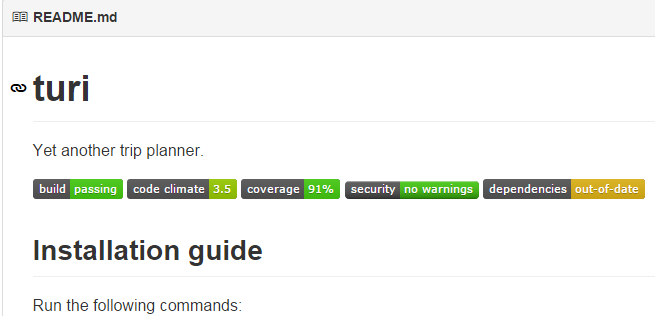
\includegraphics[scale=0.7]{pictures/badges.png}
    \caption{Project Health on the GitHub Project Site}
    \label{fig:badges}
  \end{center}
\end{figure}


\subsubsection{Travis CI}
Travis CI is a hosted continuous integration service. It is integrated with GitHub and provides testing for our project. So when we created a pull request on the development branch of the Github repository, Travis would test our new code automatically and give us a clear indication if the test was passing or not. When the pull request is merged with the development branch it would be tested once again by Travis to be sure that everything was working correctly before the pull request is automatically merged with the master branch of the repository. The log from Travis is public and can be viewed here: \url{https://travis-ci.org/turi-inc/turi/builds}.

\begin{figure}[!h]
  \begin{center}
    \includegraphics[scale=0.35]{pictures/Travis_buildlog.png}
    \caption{A sample of the build logs from Travis CI}
    \label{fig:travis_log}
  \end{center}
\end{figure}


\subsubsection{Heroku}
Heroku is a cloud platform which hosts our project for free. When a pull request is merged with the master branch it's automatically pushed to Heroku. This lets us, and other people, see a preview of the project. We had some minor problem getting this to work properly because we use Sqlite3 when we develop, but Heroku does not support Sqlite3 so we set the production database to use postgres instead.

\subsubsection{CodeClimate}
This is also a 3rd party application which checks our code for test coverage, complexity and duplications. The check is done on the master branch of the repository whenever a new pull request is merged with the branch. It gives us an indication about the code health and grades our code, on the basis of test coverage, complexity and duplications. The summary of the code climate of our project can be found here: \url{https://codeclimate.com/github/turi-inc/turi}. \\
\textit{CodeClimate} also has additional features like Trends over the "health" of our code over time, and the location "hotspots" in the code. In figure \ref{fig:codeclimate} we can see three charts. The top chart displays the overall quality of the code according to code climate. We had a small breakdown at the end since we added a lot of functionality in the end and ended up with some complex or duplicated methods. We checked the issues \textit{CodeClimate} showed us and came to the conclusion that these complex or duplicated methods are totally okay in our case. The Churn vs. Quality chart displays if classes are changed very frequently. In our case we had some classes which were under heavy development during all iterations. But this also relates to only 3 classes (yellow dots).

\begin{figure}[!h]
  \begin{center}
    \includegraphics[scale=0.35]{pictures/trends_code.png}
    \caption{CodeClimate trends}
    \label{fig:codeclimate}
  \end{center}
\end{figure}

\subsubsection{Hakiri}
This 3rd party application is used to show if any of the gems are outdated, and if there are any known security flaws in the gems we use in our project. It can be applied to every open-source project for free.

\section{Group collaboration}
When we got this assignment, we formed a Google Group to share our ideas and organize ourselves. It was also used to schedule weekly two-hour scrum meetings. These meetings started with a stand-up session, where everyone talked about what they were working on, any issues they had, and what they planned to work on that week.\\

\noindent
In the sprint planning meetings, we consistently used scrum poker after we had made sure all the user stories were clear to everyone. We did not do any retrospectives apart from the ones planned in the course, with Weihai Yu. You can find the report of our first retrospective in appendix \ref{rep:retro1}.\\

\noindent
Day to day we sat together in the lab, what ever each of us were working on. This meant that if one of us had an issue, they always had someone they could ask for help without too much effort. Everyone in the group was very helpful, so this arrangement worked out perfectly. Many of the programming sessions were done in pairs, which is a great way to avoid getting stuck for too long. During the last iteration, the weekly meetings were getting shorter and more informal because we prioritized programming, and we communicated naturally on an on-demand basis.


\noindent
As we can see in Figure \ref{fig:commitgraph} we constantly developed our features except the april down related to the eastern holidays and individual exam preparations.\\

\begin{figure}[!h]
  \begin{center}
  	\makebox[\textwidth][c]{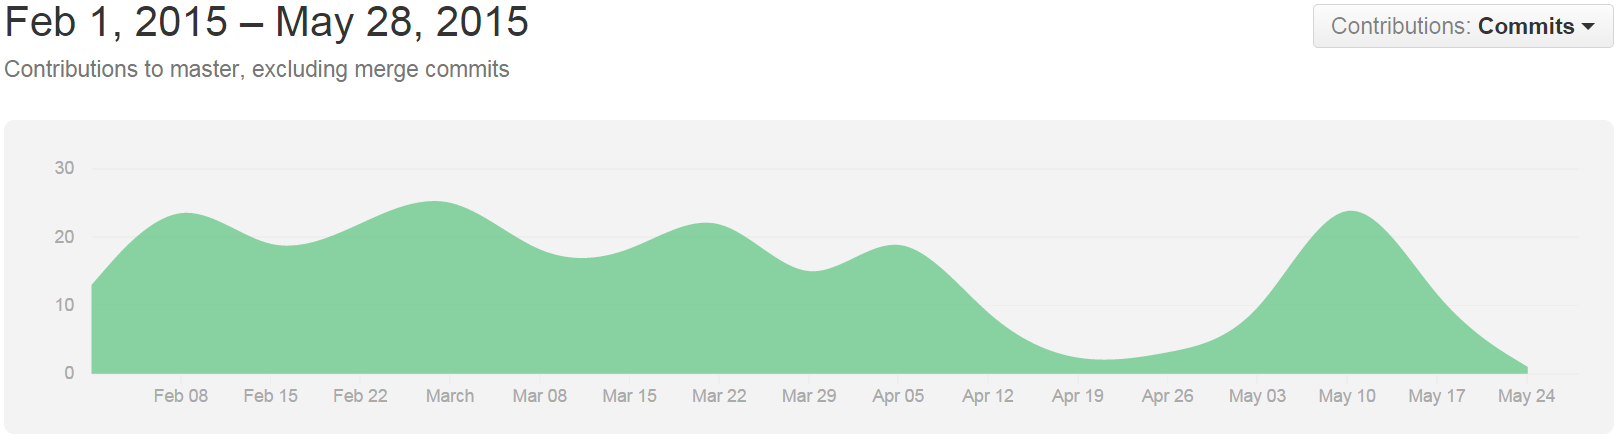
\includegraphics[width=1\textwidth]{pictures/commit_graph.png}}%
    \caption{Commit graph}
    \label{fig:commitgraph}
  \end{center}
\end{figure}

We also collected some data to show that the development of turi was spreaded over the whole week (see Figure \ref{fig:commitfrequency}). Tuesday was or weekly meeting that is why the most intensive work was done during this day. \\

\begin{figure}[!htb]
  \begin{center}
  	\makebox[\textwidth][c]{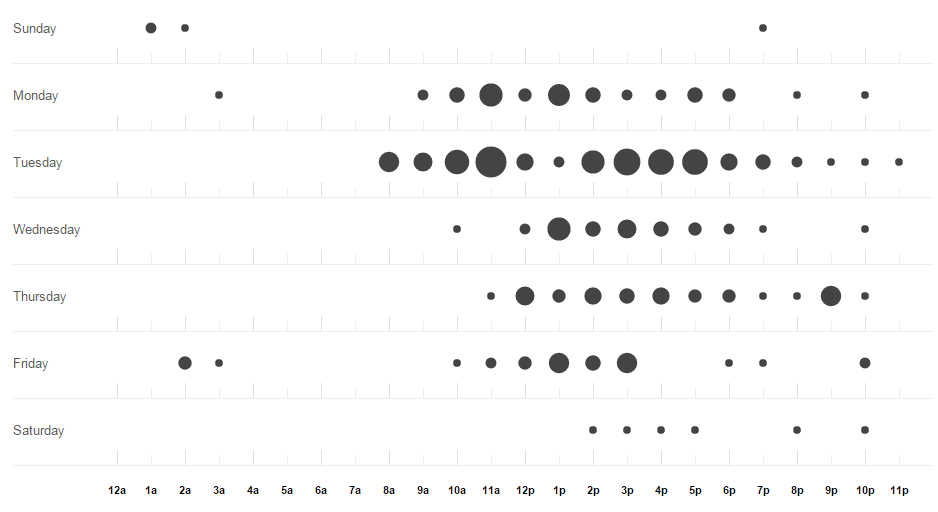
\includegraphics[width=1\textwidth]{pictures/commit_frequency.png}}%
    \caption{Commits spreading over the week}
    \label{fig:commitfrequency}
  \end{center}
\end{figure}

\section{User stories}
Our user stories are mainly related to the features we implemented. We added the user stories as appendix in table \ref{tab:sprint1}, \ref{tab:sprint2} and \ref{tab:sprint3}. As we can see in Table \ref{tab:sprint2} we reduced the number of user stories since we had to do some clean up beside that. Therefore the average sum of user story points is around 40 Points.

\section{The development process}

Using tools like GitHub and Travis CI we came up with the following workflow:

\subsection{Git Workflow}
Since we use Git together with GitHub, we are able to make use of the continuous integration tool Travis CI. Therefore we decided to go with the following development workflow. Please note that the term "origin" represents the main turi repository on GitHub.

\subsubsection{Developing of a new feature}
The developer creates a local feature branch with a telling name. A feature always relates to a user story in Agilefant.

\subsubsection{Starting a merge request}
If the developer finished with the development of his local feature, he pushes the feature branch to his own remote repository (which is a fork of the origin repository). Before he pushes his changes, he has to do a rebase on the current \textit{develop branch} of the origin to make sure all sources are up to date and we don't mess up the git history with thousands of branches. After making sure that everything is up to date, the developer can create a merge request on GitHub from his feature branch to the origin \textit{develop branch}.

\subsubsection{Validating the merge request}
After the merge request is submitted, it's open for discussion. For additional validation, Travis builds every merge request to ensure that all tests are running. If the Travis CI build is passing and the merge request can be fast forwarded (so the request was rebased) another developer can accept the merge. The person who accepts the merge should never be the owner of the merge request.

\subsubsection{Deploying to production}
As soon as a merge request is accepted, Travis CI will run again against the latest sources of the origin \textit{develop branch}. If the build is successful Travis will push the \textit{develop branch} to the \textit{master branch}. Therefore we will always have a stable version of turi on the \textit{master branch}. A developer should never push changes directly to the \textit{master branch}.\\

\noindent
After a push to the master Travis will push the code to Heroku and run the database migrations. Therefore we always have a stable snapshot version on heroku.

\subsection{Testing}
For this project we have three different layers of testing. This ensures that every aspect of our application is well tested and we will not break previous added functionality by adding a new feature. As mentioned previously, our build server (Travis CI) will take care of running those test automated.

\begin{figure}
  \begin{center}
    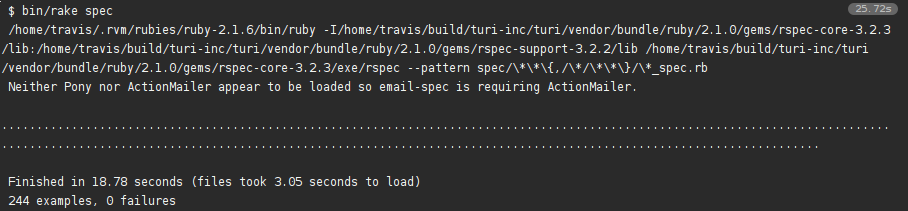
\includegraphics[scale=0.40]{pictures/rake_tests.png}
    \caption{A sample RSpec test run}
    \label{fig:}
  \end{center}
\end{figure}

\subsubsection{Model Tests}
The model tests are relatively simple and they handle the lowest level of the site, the database layer. The tests check if the database requires the appropriate fields, before saving anything to the database. We have implemented model tests for all the features, to make sure the database is consistent.
\\

\subsubsection{Controller Tests}
The controller is responsible for handling the HTTP requests. Testing the controller means making sure privilege levels are enforced, and that the CRUD operations do no more, and no less, than they are supposed to. There are tests for all of our controller functions.
\\

\subsubsection{Feature Tests}
The feature tests, are testing if the view is updated in the expected manor after a clicking a link, or doing some other action on the site it self. These test are not testing any of the underlying processes, and are not that important, though we have written feature tests for almost all of the features. 
At total we have about 240 tests, and the test coverage according to \textit{CodeClimate} is about 90 percent. \\

\section{Iterations}
\subsection{Iteration 1}
For the first iteration we focused on getting the basic features for the website working. This included authentication, participants and trip creation. We also decided on a graphical interface that would be applied to the product to make it easier to create a coherent and appealing look. Near the end of the iteration each group member went through an informal code review with an outside person. We were to explain what we had worked on, how it was done and how we tested the functionality.\\

\noindent
During development we learned that we could save time if we checked for existing gems before attempting to implement functionality from scratch. This showed up in the authentication part where we first attempted to code our own authentication system. In addition, based on the feedback from the code reviews we learned that we had to use more controller and model tests and lower the focus on feature tests.

\subsubsection{Retrospective 1}
During the first retrospective we wrote down our thoughts on the project, the group and anything relating to these. Each member wrote down their thoughts and passed the paper to their left. This continued until the papers returned at their original owners, with other members' thoughts added. The retrospect finished with the group members thanking each other for bringing something to the group. You can find the report of our first retrospective in appendix \ref{rep:retro1}.

\subsection{Iteration 2}
This iteration we decided to start implementing more and larger features. As the basic trip and authentication features were complete, the focus was on supporting features like blog and discussion platforms, maps, equipment lists, friends and an event calendar.

\subsubsection{Retrospective 2}
During the second retrospective we talked about how we were doing with various parts of the project and each member had a graph with six categories they were supposed to rate. The results showed something of a consensus for planning, development, user stories and coding. Almost everyone rated these highly, indicating these categories were handled well. Communication varied, with both high and low ratings. Some wanted more formal meetings while others thought the communication was good enough already since we usually worked in close proximity to each other and talked together while working. Documentation was rated low because we had not been creating much documentation. What we learned was that the git commits and the data from Travis also counted as documentation, meaning that we were not as lacking in this department as we first thought.

\subsection{Iteration 3}
This iteration saw very few new features. The only notable feature was an addition to the friendship system in the form of proper friend requests. We focused on finishing the features that were still unfinished at the end of iteration 2, namely the route planner and equipment lists. The main work went into making the interface design for our features coherent and doing bug fixes.


\section{Final Thoughts}

\subsection{Bjørnar}
I think the group communicated really well, and we've worked steadily, more or less from start to finish. This continuous forward momentum was really important for my motivation, as the complexity of the project increased rapidly from the get-go. Learning Ruby on Rails and JavaScript on top of HTML and Git was challenging to say the least. I'm still not sure that I really got the hang of it. I updated Agilefant somewhat diligently during the first sprint, but it quickly took the back seat as the learning curve of the other elements grew steeper. In the end I used a rough estimate to update the last two sprints. It's certainly a useful tool, but it feels a little bit clunky to interact with. Because I worked on a single user story for the entirety of the second and third sprints, I didn't need it to find out what to work on next.\\

\noindent
All that said, I appreciated the benefits of agile development, and the scrum meetings were very useful and concise. Everyone got to have their say, and the group was excellent in the sense that we didn't try to overpower each other. The user stories were well defined with acceptance criteria, so knowing \textit{what} to do was never a problem. The course as a whole has given me useful insight into the perils of software engineering and working in groups, but also into the benefits. It can be a challenge to understand other people's code, or to satisfy everyone when a decision has to be made, but the group can also be a great resource when you're stuck with a seemingly insurmountable problem.

\subsection{Florian}
In my opinion the whole group did a really, really good job. I admit, the learning curve was really high and without my previous knowledge I would have been a bit overwhelmed by the possibilities rails offers. Due to our good teamwork we managed to create an application which is nearly ready to release and could be offered a large audience. As an exchange student I really appreciated the warm welcome from my Norwegian team-mates. We had no problems to meet when it was necessary. There was a small down related to exam preparations in April but this hadn't any influence on the efficiency of our group.

\noindent
Sometimes we should stick more to the Scrum methodology but due to our limited time it was not always possible to plan the User Stories in very detail or to have something like a daily meeting (which we replaced with a "weekly").

\noindent
To sum up I felt really comfortable in this team during all iterations. We all learned new and useful things which can be used in our later work life. I would like to continue the work on our application beyond this course and try to lunch the product together with the whole team.

\subsection{Ingvild}
The communication in the group was really good, even if though we had only one formally meeting in the week. It think it was mostly because all from the group where sitting together on the same places in the lab the whole semester, so it was easy to ask anybody for help. In the beginning it was a lot to learn, since ruby was a whole new language for me and I had to learn HTML also. But after a while I got some of it, and it was really good to be able to ask the group for help on something difficult and get an answer. I think we where very lucky that Florian already could a lot ruby and could learn the rest of the group and help any group member that hadn't gotten so much hang on it in the start.\\

\noindent
The Agilefant was a useful tool for having the user story on one place, but writing down the spent time on a user story got forgotten when one worked on the user story. So my spent time is probably less than i worked, because I only wrote the time I had worked when I was finished with a user story. It probably would be more useful to use a tool one could use while also being able to work on the user story. \\

\noindent
The course itself have been really interesting, it was interesting to learn web development and to  also be able to work on a group, something that is not done in that many other courses.

\subsection{Kristoffer}
\noindent
For the first few weeks of this assignment the workload felt quite overwhelming since we had to learn so many new things before we could start the project. There was a new language, web-framework and testing framework. And by our own choice, we went ahead with the map feature, and needed to learn JavaScript, and the leaflet API as well.  
The initial shock, I think could have been alleviated if we used the Django web-framework instead, since we have used Python in previous courses.
Our group was also very lucky to have the exchange student, Florian on the team, since he was very experienced with creating web-applications. This made the project progress very fast in the beginning, but it could be a bit hard to keep up at beginning. \\

\noindent
The communication in the group may have been better organized, since we only had one formal meeting each week. However, it felt like there was good communication in the group. All the members of the group have been sitting at the same place in the lab for the whole semester, even when working with other courses, and many days the whole group was present. Thus, getting help with a problem was very easy.
From previous experiences, working in groups could be very challenging, luckily this has not been the case for this assignment, and I felt that the group worked well together. Working in scrum groups and using agile methods, has given valuable insight into software engineering.  \\

\subsection{Martin}
I think the group communication was good, the meeting each week gave us a opportunity to talk about our work and get feedback on the user stories we were working on and ask for help if we were stuck on something. By having a place to meet in the lab, gave us also the ability to ask each other questions about our code and the problem we faced during the development. \\ 
The complexity did quickly increase in the second iteration of the project, it was hard to keep up all the changes. But we all worked on our own features so we didn't have to keep up with all the changes, so I think it worked out fine. \\
As for Agilefant I think it's a useful tool, but it was really easy to forget to update. Therefore some of the user stories have a estimates time used. \\

\noindent
As for the course itself, it was quite interesting to learn web development, Ruby-on-Rails, Git and agile development. It's something completely different from the things we're done in the past. In addition to the the language and the version-control we also had to learn bootstrap, how to use the AppUI elements, how to design a HTML view and some basic JavaScript. 

\subsection{Ole-Morten}
\noindent
During the first sprint, the complexity of the product seemed overwhelming. It was difficult to get a realistic grasp on how much work needed to be done, and it was hard to look past the feeling of having taken on a project too big to finish. The early implementation of the graphical interface also created some issues when coding as the html code for the interface represented another thing to learn on top of Ruby and Rails. As features were completed and I started getting an idea of how much time went into developing each feature the project, while still complex, seemed less insurmountable.\\

\noindent
How the various tasks were divided among the group members seemed to work out pretty well, although some may have required more effort than expected. I ended up with the smaller tasks, like search and blogs, which ended up as a good thing since I struggled with understanding Rails. Quite a bit of time was spent on reading and understanding how things were supposed to work. Getting comfortable with the tools also took some time. We used git for version control and while I had some experience with simple git usage, the way we worked with it was unfamiliar. It took some time getting comfortable working with the git setup without worrying about doing something wrong. Considering the Agilefant tool, it differed how extensively group members used it and personally I never got to the point where I properly understood how to use the tool outside of adding time spent on user stories. I never felt like I had to learn more about it either since other members usually added and updated the user stories.\\

\noindent
Generally working in groups and collaborating is always a challenge, especially for someone timid, but in the end it worked out well.

\subsection{Runar}
I, as most of the other in the group, was overwhelmed by the amount of new things to learn at the beginning of this course. Most of the technologies we used, such as Ruby, Rails, html, css and javascript, I didn't have any experience using in development. By reading the ``Rails 4 in Action'' book \cite{railsaction} I got a good introduction to the web framework, but it was still hard to get it to work in practice. During the first iteration I used most of my time trying to understand how the framework worked and how to use the different technologies together. It was good that we as a group worked together to learn. \\

\noindent
In the second iteration I was understanding more and felt I could contribute more to the implementation of the features. Me and Ingvild pair programmed two features together during the second and third iteration. We used the pomodoro technique \cite{pomodoro}, which means we made a list of things to implement the next 25 minutes and then we started working hard together to complete these things. After 25 minutes we had a 5 minute break. Then we repeated the pattern. This worked very good for us and we got a boost in productivity.

\printbibliography[heading=bibintoc, title={References}]

% \begin{thebibliography}{9}

% \bibitem{puma}
% \emph{Puma webserver - GitHub}\\
% \url{https://github.com/puma/puma}

% \bibitem{heroku}
% \emph{Heroku Ruby webserver advise}\\
% \url {https://devcenter.heroku.com/articles/ruby-default-web-server}

% \bibitem{devise}
% \emph{Devise - GitHub}\\
% \url{https://github.com/plataformatec/devise}

% \bibitem{pundit}
% \emph{Pundit - GitHub}\\
% \url{https://github.com/elabs/pundit}

% \bibitem{leaflet}
% \emph{Leaflet JS}\\
% \url{http://leafletjs.com/}

% \bibitem{ckeditor}
% \emph{CKEditor}\\
% \url{https://en.wikipedia.org/wiki/CKEditor}

% \bibitem{kaminari}
% \emph{Kaminari - GitHub}\\
% \url{https://github.com/amatsuda/kaminari}

% \end{thebibliography}

\pagebreak
\appendix

\section{User Stories}
\label{sec:user-stories}

\begin{table}[H]
  \begin{tabulary}{1.0\textwidth}{|L|L|L|}
    \hline
    N. & User story & Pts \\ \hline
    
    1&As a user, I want to look at the website during the development, so that I can see the progress.
    & 5 \\ \hline
    
    2&As a user, I want to be able to register on the web page, so that I can login into the planner.
    & 5 \\ \hline

    3&As a logged in user, I want to be able to see my account page, so that I can get an overview of my activity and information.
    & 5 \\ \hline

    4&As a logged in user, I want to create a trip, so that I can plan it. 
    & 8 \\ \hline

    5&As a registerd user, I want to be able to log in and start a session, and log out, to prevent access to my personal data. & 3 \\ \hline

    6&As an owner of a trip, I want to be able to edit the details, so that I can redo or add information. & 5 \\ \hline

    7&As a logged in user, I want to be able to see a details page of my trip, so that I can display the details of my trip. & 3 \\ \hline

    8&As an owner of a trip, I want to be able to delete the trip, so that I can delete my data because I am not planning on going anyway. & 3 \\ \hline

    9&As a User I want to be able to share my trips (like the google drive sharing model) & 8 \\ \hline

    10&As a user I want to be able to search for trips so that I can easily look up relevant trips. & 8 \\ \hline
    &SUM & 53 \\ \hline
  \end{tabulary}
  \caption{Sprint 1 user stories}
\end{table}

\begin{table}[H]
  \centering
  \begin{tabulary}{1.0\textwidth}{|L|L|L|}
    \hline
    N. & User story & Pts \\ \hline

    1&As a trip user I want to be able to create events for my trip so that I can organize my trip with the other participant.
    & 5 \\ \hline

    2&As a trip user I want to be able to connect my trip with a dropbox folder to show the other participants the pictures on it
    & 8 \\ \hline

    3 &As a User I want to be able to create and manage an equipment list for my trip. 
    & 8 \\ \hline

    4 & As a User I want to be able to assign equipment Items to a user (to mark that he has bought it e.g.).
    & 5 \\ \hline

    5& As a trip owner or editor I want to be able to create blog articles so that I can share my trip experience or planning results
    & 5 \\ \hline

    6& As a person I want to share turi on social networks so that my friends or other people get to know the site.
    & 1 \\ \hline

    7& As a user I want to be able to reset my password so that I can login, because I forgot my password.
    &5 \\ \hline

    8& As a Trip User I want to be able to have a discussion forum for my trip.
    & 8 \\ \hline

    9& As a user I want to explore trips using a map.
    & 8 \\ \hline

    &SUM&53 \\ \hline

    
  \end{tabulary}
  \caption{Sprint 2 user stories}
\label{tab:sprint2}
\end{table}

\begin{table}[H]
  \centering
  \begin{tabulary}{1.0\linewidth}{|L|L|L|}
    \hline
    N. & User story & Pts \\ \hline
    1& As a developer I want to have a clean code structure.
    & 5 \\ \hline

    2& As a user I want to have a uniform user interface.
    & 5 \\ \hline

    3& As a user I want to be able to set the privacy of my trip to public or private.
    & 3 \\ \hline

    4&As a user I want to manage my friends so I can stay in touch with my friends on the site.
    & 5 \\ \hline

    5& As a Trip User I want to be able to create maps with different routes using waypoints for a trip.
    & 13 \\ \hline

    & SUM & 31 \\ \hline
  \end{tabulary}
  \caption{Sprint 3 user stories}
\label{tab:sprint3}
\end{table}


\begin{landscape}
\section{Time lists}

\subsection{Meetings}
\begin{center}
\begin{tabular}{|l|l|l|l|l|l|}
\hline
\textbf{Project} & \textbf{Task Id} & \textbf{Task}  & \textbf{User} & \textbf{Date} & \textbf{Spent effort (hours)} \\ \hline
Meetings &  359 & Group Meeting 23/06 & Everyone & \multicolumn{1}{r|}{23.06.2015 11:15} & \multicolumn{1}{r|}{14.00} \\ \hline
Meetings &  358 & Group Meeting 16/06 & Everyone & \multicolumn{1}{r|}{16.06.2015 11:15} & \multicolumn{1}{r|}{14.00} \\ \hline
Meetings &  357 & Group Meeting 09/06 & Everyone & \multicolumn{1}{r|}{09.06.2015 11:15} & \multicolumn{1}{r|}{14.00} \\ \hline
Meetings &  356 & Group Meeting 02/06 & Everyone & \multicolumn{1}{r|}{02.06.2015 11:15} & \multicolumn{1}{r|}{14.00} \\ \hline
Meetings &  355 & Group Meeting 26/05 & Everyone & \multicolumn{1}{r|}{26.05.2015 11:15} & \multicolumn{1}{r|}{14.00} \\ \hline
Meetings &  354 & Group Meeting 19/05 & Everyone & \multicolumn{1}{r|}{19.05.2015 11:15} & \multicolumn{1}{r|}{14.00} \\ \hline
Meetings &  353 & Group Meeting 12/05 & Everyone & \multicolumn{1}{r|}{12.05.2015 11:15} & \multicolumn{1}{r|}{14.00} \\ \hline
Meetings &  352 & Group Meeting 05/05 & Everyone & \multicolumn{1}{r|}{05.05.2015 11:15} & \multicolumn{1}{r|}{14.00} \\ \hline
Meetings &  351 & Group Meeting 28/04 & Everyone & \multicolumn{1}{r|}{28.04.2015 11:15} & \multicolumn{1}{r|}{14.00} \\ \hline
Meetings &  350 & Group Meeting 21/04 & Everyone & \multicolumn{1}{r|}{21.04.2015 11:15} & \multicolumn{1}{r|}{14.00} \\ \hline
Meetings &  349 & Group Meeting 14/04 & Everyone & \multicolumn{1}{r|}{14.04.2015 11:15} & \multicolumn{1}{r|}{14.00} \\ \hline
Meetings &  348 & Group Meeting 07/04 & Everyone & \multicolumn{1}{r|}{07.04.2015 11:15} & \multicolumn{1}{r|}{14.00} \\ \hline
Meetings &  347 & Group Meeting 01/04 & Everyone & \multicolumn{1}{r|}{01.04.2015 11:15} & \multicolumn{1}{r|}{14.00} \\ \hline
Meetings &  346 & Group Meeting 24/03 & Everyone & \multicolumn{1}{r|}{24.03.2015 11:15} & \multicolumn{1}{r|}{14.00} \\ \hline
Meetings &  345 & Group Meeting 17/03 & Everyone & \multicolumn{1}{r|}{17.03.2015 11:15} & \multicolumn{1}{r|}{14.00} \\ \hline
Meetings &  344 & Group Meeting 10/03 & Everyone & \multicolumn{1}{r|}{10.03.2015 11:15} & \multicolumn{1}{r|}{14.00} \\ \hline
Meetings &  343 & Group Meeting 03/03 & Everyone & \multicolumn{1}{r|}{03.03.2015 11:15} & \multicolumn{1}{r|}{14.00} \\ \hline
Meetings &  342 & Group Meeting 24/02 & Everyone & \multicolumn{1}{r|}{24.02.2015 11:15} & \multicolumn{1}{r|}{14.00} \\ \hline
Meetings &  341 & Group Meeting 17/02 & Everyone & \multicolumn{1}{r|}{17.02.2015 11:15} & \multicolumn{1}{r|}{14.00} \\ \hline
Meetings &  340 & Group Meeting 10/02 & Everyone & \multicolumn{1}{r|}{10.02.2015 11:15} & \multicolumn{1}{r|}{7.00} \\ \hline
Meetings &  38 & Group Meeting 04/02 & Everyone & \multicolumn{1}{r|}{04.02.2015 11:15} & \multicolumn{1}{r|}{7.00} \\ \hline
Meetings &  4 & Group Meeting 03/02 & Everyone & \multicolumn{1}{r|}{03.02.2015 11:15} & \multicolumn{1}{r|}{14.00} \\ \hline
Meetings &  3 & Group Meeting 28/01 & Everyone & \multicolumn{1}{r|}{28.01.2015 11:15} & \multicolumn{1}{r|}{14.00} \\ \hline
Meetings &  5 & Group Meeting 21/01 & Everyone & \multicolumn{1}{r|}{21.01.2015 11:15} & \multicolumn{1}{r|}{14.00} \\ \hline
\end{tabular}
\end{center}


\subsection{Bjørnar}
\begin{tabular}{|l|l|l|l|r|r|}
\hline
\textbf{Iteration} & \textbf{Story Id} & \textbf{Comment} & \textbf{User} & \multicolumn{1}{l|}{\textbf{Date}} & \multicolumn{1}{l|}{\textbf{Spent effort (hours)}} \\ \hline
1. Sprint & 52 & Finished the account registration & Bjørnar Grøholt Prytz & 10.02.2015 18:04 & 2.00 \\ \hline
3. Sprint & 171 &  & Bjørnar Grøholt Prytz & 16.05.2015 15:44 & 4.00 \\ \hline
3. Sprint & 171 &  & Bjørnar Grøholt Prytz & 15.05.2015 15:44 & 4.00 \\ \hline
3. Sprint & 171 &  & Bjørnar Grøholt Prytz & 14.05.2015 15:49 & 4.00 \\ \hline
3. Sprint & 171 &  & Bjørnar Grøholt Prytz & 29.04.2015 15:48 & 4.00 \\ \hline
3. Sprint & 171 &  & Bjørnar Grøholt Prytz & 10.04.2015 15:43 & 4.00 \\ \hline
3. Sprint & 171 &  & Bjørnar Grøholt Prytz & 09.04.2015 15:43 & 4.00 \\ \hline
3. Sprint & 171 &  & Bjørnar Grøholt Prytz & 07.04.2015 15:43 & 4.00 \\ \hline
3. Sprint & 171 &  & Bjørnar Grøholt Prytz & 19.03.2015 15:46 & 4.00 \\ \hline
3. Sprint & 171 &  & Bjørnar Grøholt Prytz & 18.03.2015 15:43 & 4.00 \\ \hline
3. Sprint & 171 &  & Bjørnar Grøholt Prytz & 16.03.2015 15:46 & 4.00 \\ \hline
3. Sprint & 171 &  & Bjørnar Grøholt Prytz & 13.03.2015 15:46 & 4.00 \\ \hline
3. Sprint & 171 &  & Bjørnar Grøholt Prytz & 11.03.2015 15:45 & 4.00 \\ \hline
3. Sprint & 171 &  & Bjørnar Grøholt Prytz & 10.03.2015 15:41 & 4.00 \\ \hline
3. Sprint & 171 &  & Bjørnar Grøholt Prytz & 07.03.2015 15:42 & 4.00 \\ \hline
3. Sprint & 171 &  & Bjørnar Grøholt Prytz & 05.03.2015 15:41 & 4.00 \\ \hline
3. Sprint & 171 &  & Bjørnar Grøholt Prytz & 04.03.2015 15:41 & 4.00 \\ \hline
3. Sprint & 171 &  & Bjørnar Grøholt Prytz & 27.02.2015 15:40 & 4.00 \\ \hline
3. Sprint & 171 &  & Bjørnar Grøholt Prytz & 26.02.2015 15:39 & 4.00 \\ \hline
3. Sprint & 171 &  & Bjørnar Grøholt Prytz & 24.02.2015 15:38 & 4.00 \\ \hline
3. Sprint & 171 &  & Bjørnar Grøholt Prytz & 21.02.2015 15:39 & 4.00 \\ \hline
 & & & &\textbf{TOTAL}: & \textbf{127} \\ \hline
\end{tabular}

\subsection{Florian}
\begin{tabular}{|l|l|l|l|r|r|}
\hline
\textbf{Iteration} & \textbf{Story Id} & \textbf{Comment} & \textbf{User} & \multicolumn{1}{l|}{\textbf{Date}} & \multicolumn{1}{l|}{\textbf{Spent effort (hours)}} \\ \hline
1. Sprint & 152 & RSpec and Authorization & Florian Sauter & 24.02.2015 09:15 & 8.00 \\ \hline
1. Sprint & 152 & Started implementation & Florian Sauter & 20.02.2015 17:19 & 3.00 \\ \hline
1. Sprint & 78 & Theme & Florian Sauter & 17.02.2015 10:39 & 1.00 \\ \hline
1. Sprint & 70 & Theme & Florian Sauter & 17.02.2015 10:38 & 1.00 \\ \hline
1. Sprint & 66 & Logout Button and stuff & Florian Sauter & 17.02.2015 10:39 & 0.50 \\ \hline
1. Sprint & 50 & More work on Heroku and Travis and the Theme & Florian Sauter & 17.02.2015 10:38 & 5.00 \\ \hline
1. Sprint & 50 & Setup & Florian Sauter & 10.02.2015 10:28 & 4.00 \\ \hline
1. Sprint & 87 & Theme for editing & Florian Sauter & 17.02.2015 10:40 & 0.50 \\ \hline
1. Sprint & 52 & devise & Florian Sauter & 24.02.2015 11:52 & 3.00 \\ \hline
1. Sprint & 52 & Theme & Florian Sauter & 17.02.2015 10:39 & 1.00 \\ \hline
2. Sprint & 10 & Including Landing page & Florian Sauter & 02.04.2015 19:52 & 5.00 \\ \hline
2. Sprint & 247 &  & Florian Sauter & 22.04.2015 12:43 & 5.00 \\ \hline
2. Sprint & 172 & View updates (Theme) & Florian Sauter & 07.05.2015 19:50 & 4.00 \\ \hline
2. Sprint & 154 & View updates no 2. & Florian Sauter & 08.04.2015 13:00 & 6.00 \\ \hline
2. Sprint & 154 & View updates & Florian Sauter & 03.03.2015 20:54 & 5.00 \\ \hline
2. Sprint & 154 & Test prepartion & Florian Sauter & 03.03.2015 20:53 & 3.00 \\ \hline
2. Sprint & 211 & Improvements & Florian Sauter & 17.03.2015 16:27 & 2.00 \\ \hline
2. Sprint & 211 & Finalization & Florian Sauter & 08.03.2015 03:41 & 3.00 \\ \hline
2. Sprint & 211 & Improvements & Florian Sauter & 07.03.2015 23:17 & 3.00 \\ \hline
2. Sprint & 211 & First tests/implementation & Florian Sauter & 05.03.2015 16:00 & 6.00 \\ \hline
2. Sprint & 212 & Further improvements & Florian Sauter & 24.03.2015 09:40 & 3.00 \\ \hline
2. Sprint & 212 & Improvements & Florian Sauter & 17.03.2015 16:28 & 1.00 \\ \hline
2. Sprint & 212 & Implementation of Tests \& Views & Florian Sauter & 11.03.2015 12:38 & 6.00 \\ \hline
2. Sprint & 212 & Prepartion of view files & Florian Sauter & 10.02.2015 16:28 & 2.00 \\ \hline
3. Sprint & 280 & Code clean up (summoned) & Florian Sauter & 15.05.2015 12:50 & 10.00 \\ \hline
3. Sprint & 231 & Cleaned up the request and friendship controller & Florian Sauter & 18.05.2015 12:51 & 6.00 \\ \hline
3. Sprint & 231 & Updated the user page view & Florian Sauter & 15.05.2015 12:51 & 6.00 \\ \hline
3. Sprint & 279 & General improvements. & Florian Sauter & 08.05.2015 12:48 & 6.00 \\ \hline
3. Sprint & 279 & Discussion Form & Florian Sauter & 05.05.2015 12:48 & 4.00 \\ \hline
 & & & &\textbf{TOTAL}: & \textbf{157} \\ \hline
\end{tabular}


\subsection{Ingvild}
\begin{tabular}{|l|l|l|l|r|r|}
\hline
\textbf{Iteration} & \textbf{Story Id} & \textbf{Comment} & \textbf{User} & \multicolumn{1}{l|}{\textbf{Date}} & \multicolumn{1}{l|}{\textbf{Spent effort (hours)}} \\ \hline
1. Sprint & 62 &  & Ingvild Kristiane Myrvang & 27.02.2015 10:01 & 3.00 \\ \hline
1. Sprint & 52 & created register page & Ingvild Kristiane Myrvang & 08.02.2015 17:31 & 3.00 \\ \hline
3. Sprint & 231 &  & Ingvild Kristiane Myrvang & 14.05.2015 15:19 & 3.00 \\ \hline
3. Sprint & 231 &  & Ingvild Kristiane Myrvang & 12.05.2015 15:20 & 3.00 \\ \hline
3. Sprint & 231 &  & Ingvild Kristiane Myrvang & 10.05.2015 15:21 & 3.00 \\ \hline
3. Sprint & 231 &  & Ingvild Kristiane Myrvang & 07.05.2015 15:19 & 3.00 \\ \hline
3. Sprint & 231 &  & Ingvild Kristiane Myrvang & 03.05.2015 15:22 & 3.00 \\ \hline
3. Sprint & 231 &  & Ingvild Kristiane Myrvang & 13.04.2015 16:30 & 2.50 \\ \hline
3. Sprint & 231 &  & Ingvild Kristiane Myrvang & 07.04.2015 15:30 & 3.00 \\ \hline
3. Sprint & 231 &  & Ingvild Kristiane Myrvang & 25.03.2015 15:46 & 2.00 \\ \hline
3. Sprint & 231 &  & Ingvild Kristiane Myrvang & 24.03.2015 11:10 & 1.00 \\ \hline
3. Sprint & 231 &  & Ingvild Kristiane Myrvang & 19.03.2015 09:40 & 3.00 \\ \hline
3. Sprint & 231 &  & Ingvild Kristiane Myrvang & 17.03.2015 09:41 & 3.00 \\ \hline
3. Sprint & 231 &  & Ingvild Kristiane Myrvang & 16.03.2015 09:53 & 3.00 \\ \hline
3. Sprint & 231 &  & Ingvild Kristiane Myrvang & 15.03.2015 09:40 & 3.00 \\ \hline
3. Sprint & 231 &  & Ingvild Kristiane Myrvang & 13.03.2015 09:53 & 3.00 \\ \hline
3. Sprint & 231 &  & Ingvild Kristiane Myrvang & 12.03.2015 09:43 & 3.00 \\ \hline
 & & & &\textbf{TOTAL}: & \textbf{92.5} \\ \hline
\end{tabular}

\subsection{Kristoffer}
\begin{tabular}{|l|l|l|l|r|r|}
\hline
\textbf{Iteration} & \textbf{Story Id} & \textbf{Comment} & \textbf{User} & \multicolumn{1}{l|}{\textbf{Date}} & \multicolumn{1}{l|}{\textbf{Spent effort (hours)}} \\ \hline
1. Sprint & 66 &  & Kristoffer Myrseth Severinsen & 10.02.2015 18:07 & 3.00 \\ \hline
1. Sprint & 52 & Finished the account registration & Kristoffer Myrseth Severinsen & 10.02.2015 18:04 & 2.00 \\ \hline
3. Sprint & 171 &  & Kristoffer Myrseth Severinsen & 18.05.2015 15:45 & 4.00 \\ \hline
3. Sprint & 171 &  & Kristoffer Myrseth Severinsen & 15.05.2015 15:44 & 4.00 \\ \hline
3. Sprint & 171 &  & Kristoffer Myrseth Severinsen & 14.05.2015 15:49 & 4.00 \\ \hline
3. Sprint & 171 &  & Kristoffer Myrseth Severinsen & 29.04.2015 15:48 & 4.00 \\ \hline
3. Sprint & 171 &  & Kristoffer Myrseth Severinsen & 10.04.2015 15:43 & 4.00 \\ \hline
3. Sprint & 171 &  & Kristoffer Myrseth Severinsen & 09.04.2015 15:43 & 4.00 \\ \hline
3. Sprint & 171 &  & Kristoffer Myrseth Severinsen & 07.04.2015 15:43 & 4.00 \\ \hline
3. Sprint & 171 &  & Kristoffer Myrseth Severinsen & 19.03.2015 15:46 & 4.00 \\ \hline
3. Sprint & 171 &  & Kristoffer Myrseth Severinsen & 18.03.2015 15:43 & 4.00 \\ \hline
3. Sprint & 171 &  & Kristoffer Myrseth Severinsen & 16.03.2015 15:46 & 4.00 \\ \hline
3. Sprint & 171 &  & Kristoffer Myrseth Severinsen & 13.03.2015 15:46 & 4.00 \\ \hline
3. Sprint & 171 &  & Kristoffer Myrseth Severinsen & 11.03.2015 15:45 & 4.00 \\ \hline
3. Sprint & 171 &  & Kristoffer Myrseth Severinsen & 10.03.2015 15:41 & 4.00 \\ \hline
3. Sprint & 171 &  & Kristoffer Myrseth Severinsen & 07.03.2015 15:42 & 4.00 \\ \hline
3. Sprint & 171 &  & Kristoffer Myrseth Severinsen & 05.03.2015 15:41 & 4.00 \\ \hline
3. Sprint & 171 &  & Kristoffer Myrseth Severinsen & 04.03.2015 15:41 & 4.00 \\ \hline
3. Sprint & 171 &  & Kristoffer Myrseth Severinsen & 27.02.2015 15:40 & 4.00 \\ \hline
3. Sprint & 171 &  & Kristoffer Myrseth Severinsen & 26.02.2015 15:39 & 4.00 \\ \hline
3. Sprint & 171 &  & Kristoffer Myrseth Severinsen & 24.02.2015 15:38 & 4.00 \\ \hline
3. Sprint & 171 &  & Kristoffer Myrseth Severinsen & 21.02.2015 15:39 & 4.00 \\ \hline
 & & & &\textbf{TOTAL}: & \textbf{130} \\ \hline
\end{tabular}

\subsection{Martin}
\begin{tabular}{|l|l|l|l|r|r|}
\hline
\textbf{Iteration} & \textbf{Story Id} & \textbf{Comment} & \textbf{User} & \multicolumn{1}{l|}{\textbf{Date}} & \multicolumn{1}{l|}{\textbf{Spent effort (hours)}} \\ \hline
1. Sprint & 152 & Started implementation & Martin Mikalsen & 20.02.2015 17:19 & 3.00 \\ \hline
1. Sprint & 78 &  & Martin Mikalsen & 10.02.2015 18:10 & 3.00 \\ \hline
1. Sprint & 70 & Controller test & Martin Mikalsen & 03.03.2015 16:18 & 3.00 \\ \hline
1. Sprint & 70 &  & Martin Mikalsen & 10.02.2015 18:09 & 4.00 \\ \hline
1. Sprint & 66 &  & Martin Mikalsen & 10.02.2015 18:09 & 3.00 \\ \hline
1. Sprint & 50 & Helping :3  & Martin Mikalsen & 10.02.2015 18:01 & 4.00 \\ \hline
1. Sprint & 92 &  & Martin Mikalsen & 10.02.2015 18:09 & 2.00 \\ \hline
1. Sprint & 87 & refactoring test & Martin Mikalsen & 24.02.2015 11:52 & 2.00 \\ \hline
1. Sprint & 87 &  & Martin Mikalsen & 10.02.2015 18:06 & 3.00 \\ \hline
1. Sprint & 52 & devise & Martin Mikalsen & 24.02.2015 11:51 & 2.00 \\ \hline
2. Sprint & 155 & Updated view & Martin Mikalsen & 04.04.2015 19:00 & 4.00 \\ \hline
2. Sprint & 155 & Mostly done & Martin Mikalsen & 31.03.2015 19:35 & 7.00 \\ \hline
2. Sprint & 155 & views/controller & Martin Mikalsen & 30.03.2015 19:35 & 4.00 \\ \hline
2. Sprint & 155 & Model, controller and some tests made & Martin Mikalsen & 18.03.2015 10:14 & 4.00 \\ \hline
2. Sprint & 155 & Implemnting & Martin Mikalsen & 17.03.2015 19:35 & 5.00 \\ \hline
2. Sprint & 154 & Charts & Martin Mikalsen & 08.04.2015 13:29 & 12.00 \\ \hline
2. Sprint & 154 & Continue on implenation & Martin Mikalsen & 11.03.2015 12:13 & 7.00 \\ \hline
2. Sprint & 154 & Started with Equipment item & Martin Mikalsen & 06.03.2015 09:37 & 7.00 \\ \hline
2. Sprint & 154 & Controller, view and controller tests & Martin Mikalsen & 04.03.2015 18:52 & 7.00 \\ \hline
2. Sprint & 154 & Started creating the equipment list & Martin Mikalsen & 03.03.2015 20:52 & 6.00 \\ \hline
3. Sprint & 280 & Clean up & Martin Mikalsen & 28.05.2015 19:47 & 2.00 \\ \hline
3. Sprint & 231 & Cleaned up the request and friendship controller  & Martin Mikalsen & 18.05.2015 12:52 & 6.00 \\ \hline
3. Sprint & 231 & updated the user page view & Martin Mikalsen & 15.05.2015 12:42 & 6.00 \\ \hline
3. Sprint & 278 & Approximation timed used... & Martin Mikalsen & 24.05.2015 20:31 & 12.00 \\ \hline
 & & & &\textbf{TOTAL}: & \textbf{165} \\ \hline
\end{tabular}




\subsection{Ole-Morten}
\begin{tabular}{|l|l|l|l|r|r|}
\hline
\textbf{Iteration} & \textbf{Story Id} & \textbf{Comment} & \textbf{User} & \multicolumn{1}{l|}{\textbf{Date}} & \multicolumn{1}{l|}{\textbf{Spent effort (hours)}} \\ \hline
1. Sprint & 151 &  & Ole-Morten Tangen & 27.02.2015 12:21 & 2.00 \\ \hline
1. Sprint & 151 &  & Ole-Morten Tangen & 23.02.2015 12:19 & 6.00 \\ \hline
1. Sprint & 151 &  & Ole-Morten Tangen & 20.02.2015 12:12 & 6.00 \\ \hline
1. Sprint & 151 &  & Ole-Morten Tangen & 19.02.2015 12:18 & 4.00 \\ \hline
1. Sprint & 151 &  & Ole-Morten Tangen & 18.02.2015 12:18 & 6.00 \\ \hline
1. Sprint & 52 & Finished the account registration & Ole-Morten Tangen & 10.02.2015 18:04 & 2.00 \\ \hline
2. Sprint & 206 &  & Ole-Morten Tangen & 27.03.2015 11:02 & 1.00 \\ \hline
2. Sprint & 206 &  & Ole-Morten Tangen & 25.03.2015 11:04 & 3.00 \\ \hline
2. Sprint & 206 &  & Ole-Morten Tangen & 24.03.2015 16:52 & 5.00 \\ \hline
2. Sprint & 206 &  & Ole-Morten Tangen & 17.03.2015 16:01 & 3.00 \\ \hline
2. Sprint & 206 &  & Ole-Morten Tangen & 16.03.2015 17:22 & 4.00 \\ \hline
2. Sprint & 206 &  & Ole-Morten Tangen & 13.03.2015 12:39 & 1.00 \\ \hline
2. Sprint & 206 &  & Ole-Morten Tangen & 11.03.2015 12:38 & 2.00 \\ \hline
 & & & &\textbf{TOTAL}: & \textbf{90} \\ \hline
\end{tabular}



\subsection{Runar}
\begin{tabular}{|l|l|l|l|r|r|}
\hline
\textbf{Iteration} & \textbf{Story Id} & \textbf{Comment} & \textbf{User} & \multicolumn{1}{l|}{\textbf{Date}} & \multicolumn{1}{l|}{\textbf{Spent effort (hours)}} \\ \hline
1. Sprint & 62 &  & Runar Flåten & 28.05.2015 22:36 & 10.00 \\ \hline
2. Sprint & 177 &  & Runar Flåten & 28.05.2015 22:34 & 10.00 \\ \hline
2. Sprint & 172 &  & Runar Flåten & 28.05.2015 22:36 & 20.00 \\ \hline
3. Sprint & 231 &  & Runar Flåten & 28.05.2015 22:35 & 15.00 \\ \hline
3. Sprint & 171 &  & Runar Flåten & 28.05.2015 22:37 & 10.00 \\ \hline
3. Sprint & 279 &  & Runar Flåten & 28.05.2015 22:34 & 4.00 \\ \hline
 & & & &\textbf{TOTAL}: & \textbf{113} \\ \hline
\end{tabular}


\end{landscape}


\section{Retrospective - 1 Results}
\label{rep:retro1}

Here is an overview of the things we mentioned and the results (discussed with the teacher) for our first retrospective.

\textbf{Results}

\begin{itemize}
	\item Choose a master next meeting
	\item Make daily even if not everyone can participate (15 minutes - standup - what have i done, what problems i had, what I'm going to do)
	\item Create workshops for the things you done (just create an appointment - who can participate participates)
	\item Take more time for the next sprint planning (find an appointment next tirsdag) - at least 4 to 5 hours
\end{itemize}

\textbf{Detailed points with unfiltered comments of all:}
\begin{itemize}
	\item Things are progressing fast!
	\begin{itemize}
		\item Good
	\end{itemize}
	\item A lot was done in the first iteration
	\begin{itemize}
		\item We can do more =)
	\end{itemize}
	\item Base program, nearly done
	\begin{itemize}
		\item Suprised how fast things are stacking up
		\item Awesome
	\end{itemize}
	\item Complexity is increasing
	\begin{itemize}
		\item Knowledge too
	\end{itemize}
	\item Tests are overlapping (Model/Controller/view)
	\item Good dialog between team members
	\item Git is nice
	\begin{itemize}
		\item Yes but very complicated also sometimes
		\item + Annoying but better thean CVS/SVN :P
	\end{itemize}
	\item Continuous Integration/delivery is also very nice
	\item We have a good team atmosphere
	\begin{itemize}
		\item Our team is ze best
	\end{itemize}
	\item Good collaboration which can be extended
	\begin{itemize}
		\item Party/do things outside school?
		\item Yes I'd like a Party!
	\end{itemize}
	\item More pair programming
	\begin{itemize}
		\item Yes and switch it up!
	\end{itemize}
	\item More exchange of learned things between Members!
	\begin{itemize}
		\item Maybe set an hour in the meeting explaining new features?
		\item Workshops in the group!
	\end{itemize}
	\item We should have a kanban board
	\item There should be more acceptance criterias
	\begin{itemize}
		\item Maybe set an hour in the meeting explaining new features?
		\item Workshops in the group!
	\end{itemize}
	\item We should have workshops within our group about 	such as the new gems we are using and rails, javascript, css, html etc.
	\begin{itemize}
		\item Awesome idea.
	\end{itemize}
	\item Each user story should have points, use the planning poker
	\item Our meetings should be more effective, maybe set up an agenda for each meeting
	\item We should have a motivated master which focus is on the organization part (like meeting agenda)
\end{itemize}

\end{document}

%%% Local Variables:
%%% mode: latex
%%% TeX-master: t
%%% End:
